\documentclass[a4paper, 12pt, twoside]{book}
	\PassOptionsToPackage{table}{xcolor}
	\usepackage[export]{adjustbox}
	\usepackage[english,ngerman]{babel}
	\usepackage{amsmath, url}
	\usepackage[utf8]{inputenc}
	\usepackage[dvipsnames]{xcolor}
	\usepackage[T1]{fontenc}
	\usepackage{import}
	\usepackage{graphicx}
	\usepackage{subcaption}
	\usepackage{verbatim}
	\usepackage{float}
	\usepackage[headheight=12pt]{geometry}
	\usepackage{fancyhdr}
	\usepackage{subfiles}
	\usepackage{float}
	

	%  Bibliographie
\usepackage{bibgerm} % Umlaute in BibTeX
%\usepackage[style=authortitle-icomp]{biblatex}
\bibliographystyle{abbrv} 
\usepackage[babel,german=guillemets]{csquotes}

	

	\pagestyle{fancy}
	\fancyhf{}
	\fancyhead[LE,RO]{Baran Avinc}
	\fancyhead[RE,LO]{Masterarbeit}
	\fancyfoot[LE,RO]{\vspace{0.05cm}\thepage}
	%\fancyfoot[RE,LO]{\vspace{0.05cm}
\includegraphics[width=0.1\textwidth]{Bilder/TU-Berlin-Logo.pdf}}
	\renewcommand{\headrulewidth}{1pt}
	\renewcommand{\headrule}{\hbox to\headwidth{\color{RoyalPurple}\leaders\hrule height 				\headrulewidth\hfill}}
	\renewcommand{\footrulewidth}{1pt}
	\renewcommand{\footrule}{\hbox to\headwidth{\color{RoyalPurple}\leaders\hrule height \footrulewidth\hfill}}
	\pagestyle{fancy}


	


  	%
\includegraphics[width=0.1\textwidth]{Bilder/TU-Berlin-Logo.pdf}

	





\begin{document}
	
\begin{titlepage}
		\pagestyle{fancy}
		\centering\textbf{\large Masterarbeit zum Thema}\\
		\vspace{3cm} 
		\noindent{\color{RoyalPurple}\rule{\textwidth}{1pt}} \\
		\vspace{0.5cm} 
		\centering\textbf{\large Untersuchung der optischen Polarisation und internen Quanteneffizienz von AlGaN Quantenfilmen mittels temperatur- und leistungsabhängiger Photolumineszenzspektroskopie} \\
		\vspace{0.25cm} 
		\noindent{\color{RoyalPurple}\rule{\textwidth}{1pt}} \\
		\vspace{3cm}
		\centering Baran Avinc \\
		\vspace{3cm}
		\centering Institut für Festkörperphysik
		\vspace{\fill} \\
		\raggedleft{
\includegraphics[width=0.2\textwidth]{Bilder/TU-Berlin-Logo.pdf}}
\end{titlepage}



	\tableofcontents\thispagestyle{fancy}
	
\chapter{Einleitung}
\thispagestyle{fancy}

\begin{quote}
In the spirit of Alfred Nobel the Prize rewards an invention of greatest benefit to mankind; using blue LEDs, white Light can be created in a new way.\end{quote}
Dieser Satz den die Schwedische Akademie der Künste nach der Vergabe des Nobelpreises an die Entwicklung der blauen LED(kurz, light emitting diode) im Jahr 2014 an die Presse veröffentlichte, fasst treffend zusammen, wie hoch die Bedeutung der auf Halbleiterkristallen basierenden optischen Bauelemente ist.
LEDs nehmen einen fundamentalen und immer bedeutender werdenden Teil unseres alltäglichen Lebens ein. Ausgezeichnet durch ihre hervorragende Effizienz, konkurrenzlosen Lebensdauer und geringen Dimension übernimmt sie durch eine immer höher werdenden Lichtausbeute zusehends neue Anwendungsbereiche. 
%Seit jeher etabliert in den Bereichen der optischen Datenübertragung und Leuchtanzeige schreiten immer mehr andere Wellenlängenbereiche in den Fokus der weltweiten Forschung. 
Insbesondere auf Gallium Nitrid (GaN) basierende Halbleitermaterialien haben einen bahnbrechenden Weg hingelegt, der zur Entwicklung von hoch effizienten und leuchtstarken blauen LEDs führte.




	\chapter{Grundlagen}
	\subfile{Kapitel/Grundlagen.tex}
	\subfile{Kapitel/GrundlagenPL.tex}
	\subfile{Kapitel/GrundlagenPLIQE.tex}
	\subfile{Kapitel/GrundlagenPLtrueIQE.tex}
	
\chapter{Aufbau}


\thispagestyle{fancy}
\label{chap:aufbau}
\section{Photolumineszenzaufbau}
\begin{figure}[!htb]
    \centering
    \begin{minipage}[t]{\linewidth}
        \centering
        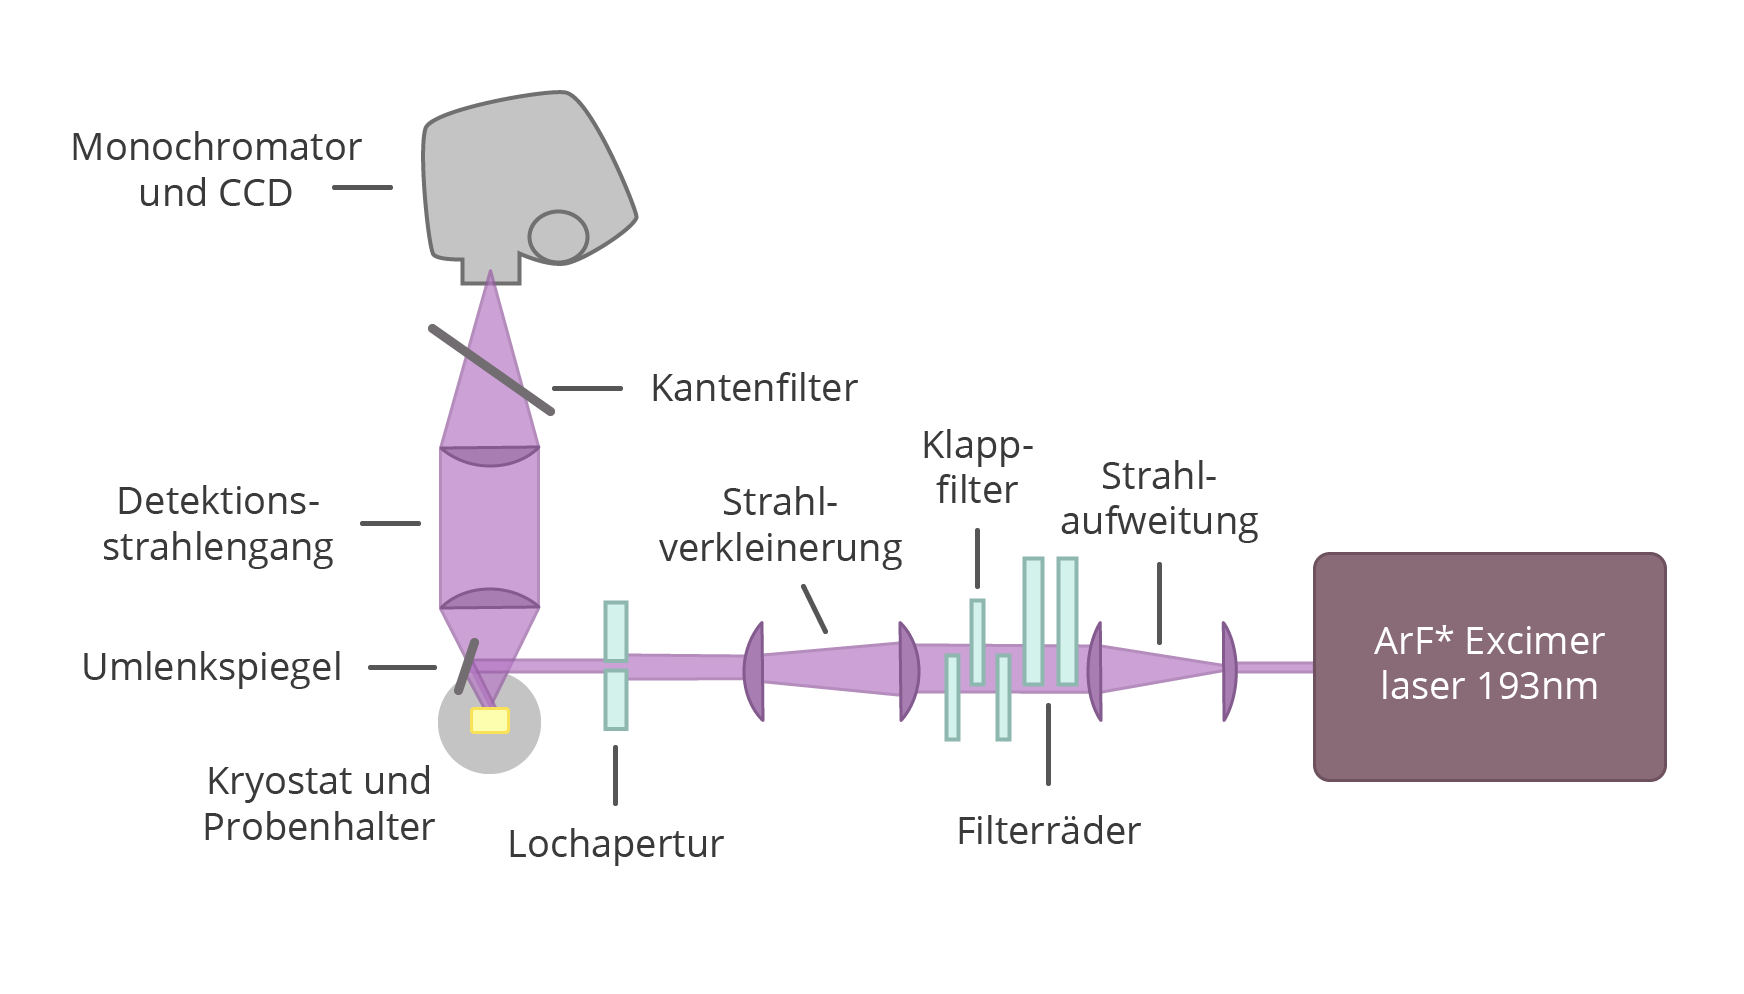
\includegraphics[width=0.8\linewidth]{Bilder/aufbauPL.png}
        \caption{Aufbau des Photolumineszenzmessplatzes der AG Kneissl. }
        \label{fig:plaufbau}
    \end{minipage}% <- sonst wird hier ein Leerzeichen eingefügt
\end{figure}
\noindent
Für die experimentelle Untersuchung der UV-Photolumineszenz wurde der PL-Aufbau der AG-Kneissl, der in Abbildung \ref{fig:plaufbau} dargestellt ist, verwendet. Der PL-Aufbau wurde von Christoph Reich in der Zeit seiner Diplomarbeit aufgebaut und während seiner Promotion erweitert \cite{creich}. 
Als Anregungsquelle für die Photolumineszenz dient ein ArF-Excimerlaser mit einer Wellenlänge von $193 \ nm$ ($6,4 \ eV$). Mit dieser Wellenlänge ist er bestens geeignet für die Überbandanregung von Nitridhalbleitern. 
Des Weiteren bietet der Aufbau die Möglichkeit von temperaturabhängigen Untersuchungen von $5 \ K $ bis $300 K$. Dies ist auch die Grundlage für die Bestimmung der IQE. 
\newline
Der Laser mit dem Modellnamen "`Xantos XS"' von der Firma Coherent bietet eine maximale Emissionsenergie von $ 5 \ mJ $ und eine einstellbare Frequenz bis zu 500 Hz bei einer Pulsdauer von $5 \ ns$.
Durch interne Rückkopplung ist eine Energiestabilisierung möglich, die die Schwankung der Anregungsleistung auf 3 Prozent minimiert. 
\newline
Die Ansteuerung des kompletten Messvorgangs erfolgt durch die Messsoftware von Christoph Reich, entwickelt in der grafischen Programmiersprache "`LabView"' von Texas Instruments. Diese ermöglicht alle nötigen Einstellungen an Pumpen, Heizern, Laser, Filtern und Spektrometer, um einen nahezu komplett automatisierten Messvorgang zu starten. Spektren können so mit verschiedenen Parametern wie Position, Anregungsleistungsdichte, Temperatur, Energiebereich und Integrationszeit aufgenommen werden und auch ein Gaswechsel ist möglich.
\newline
Beginnend vom Laser wird im ersten Schritt der Laserstrahl durch ein Linsensystem, bestehend aus einer Zerstreuungs- und Sammellinse, aufgeweitet. Dieser Schritt ermöglicht es, die Anregungsleistungsdichte zu verringern, um die am Aufbau beteiligten Geräten, insbesondere die Filterräder, nicht mit zu hohen Leistungen zu beschädigen. Mit Hilfe der Filterräder ist es möglich, die Anregungsleistungsdichte 61 stufig zu variieren und somit leistungsdichteabhängige IQE Messungen zu machen. Als nächstes passiert der Strahl ein Linsensystem aus zwei Sammellinsen für eine Strahlverkleinerung. Vor dem Auftreffen des Strahles am Probenhalter im Kryostaten passiert der Strahl noch eine Lochblende. Sie dient der Entfernung achsennaher Strahlen und um bei Bedarf den Strahldurchmesser noch weiter zu verringern. 
\newline
Um den Strahl in Richtung des Probenhalters durch das Fenster im Kryostaten zu lenken, wird ein Spiegel mit einer dielektrischen Beschichtung benutzt. Der Laserstrahl durchdringt die Fenster des Kryostaten, welche speziell für eine hohe Transmission in diesem Wellenlängenbereich ausgelegt sind. Der Kryostat selbst ist horizontal und vertikal verschiebbar, um die Messung mehrerer Proben im Probenhalter in einem Messvorgang bei gleichen Bedingungen zu ermöglichen. Die Proben werden mit einem Kleber auf dem Probenhalter selbst befestigt, bevor dieser in den Kryostaten geschoben wird. 
Die Anregung der Proben mit dem Laserstrahl führt zur probenspezifischen Emission von Licht. Diese wird von einer Linse im Strahlengang vor dem Detektor eingefangen und von einer zweiten Linse auf den Monochromatorspalt fokussiert.
\newline
Bei dem Monochromator handelt es sich um einen "`iHR 320"' des Herstellers "`Horiba"'. Zur Verfügung stehen drei Blazegitter mit $300 \thinspace \frac{Linien}{mm}$,
$600 \thinspace \frac{Linien}{mm}$ und $1800 \thinspace \frac{Linien}{mm}$. Bei der verwendeten Spaltbreite von $100 \thinspace \mu m$ entspricht die maximale Auflösung in etwa $5 \thinspace meV$ ($0,17 \thinspace nm$). Für Messungen oberhalb von $225 \thinspace nm$ besteht die Möglichkeit einen Kantenfilter in den Strahlengang einzubringen, mit dem das Laserstreulicht und dessen höhere Ordnungen aus dem Spektrum entfernt werden können. Bei dem CCD Chip handelt es sich um das Modell "`Syncerity"' von "`Horiba"' der "`open electrode"' -Bauart mit 1024x256 einzelnen Pixeln. 

\section{Messaufbau Lichtpolarisation}
\begin{figure}[!htb]
    \centering
    \begin{minipage}[t]{\linewidth}
        \centering
        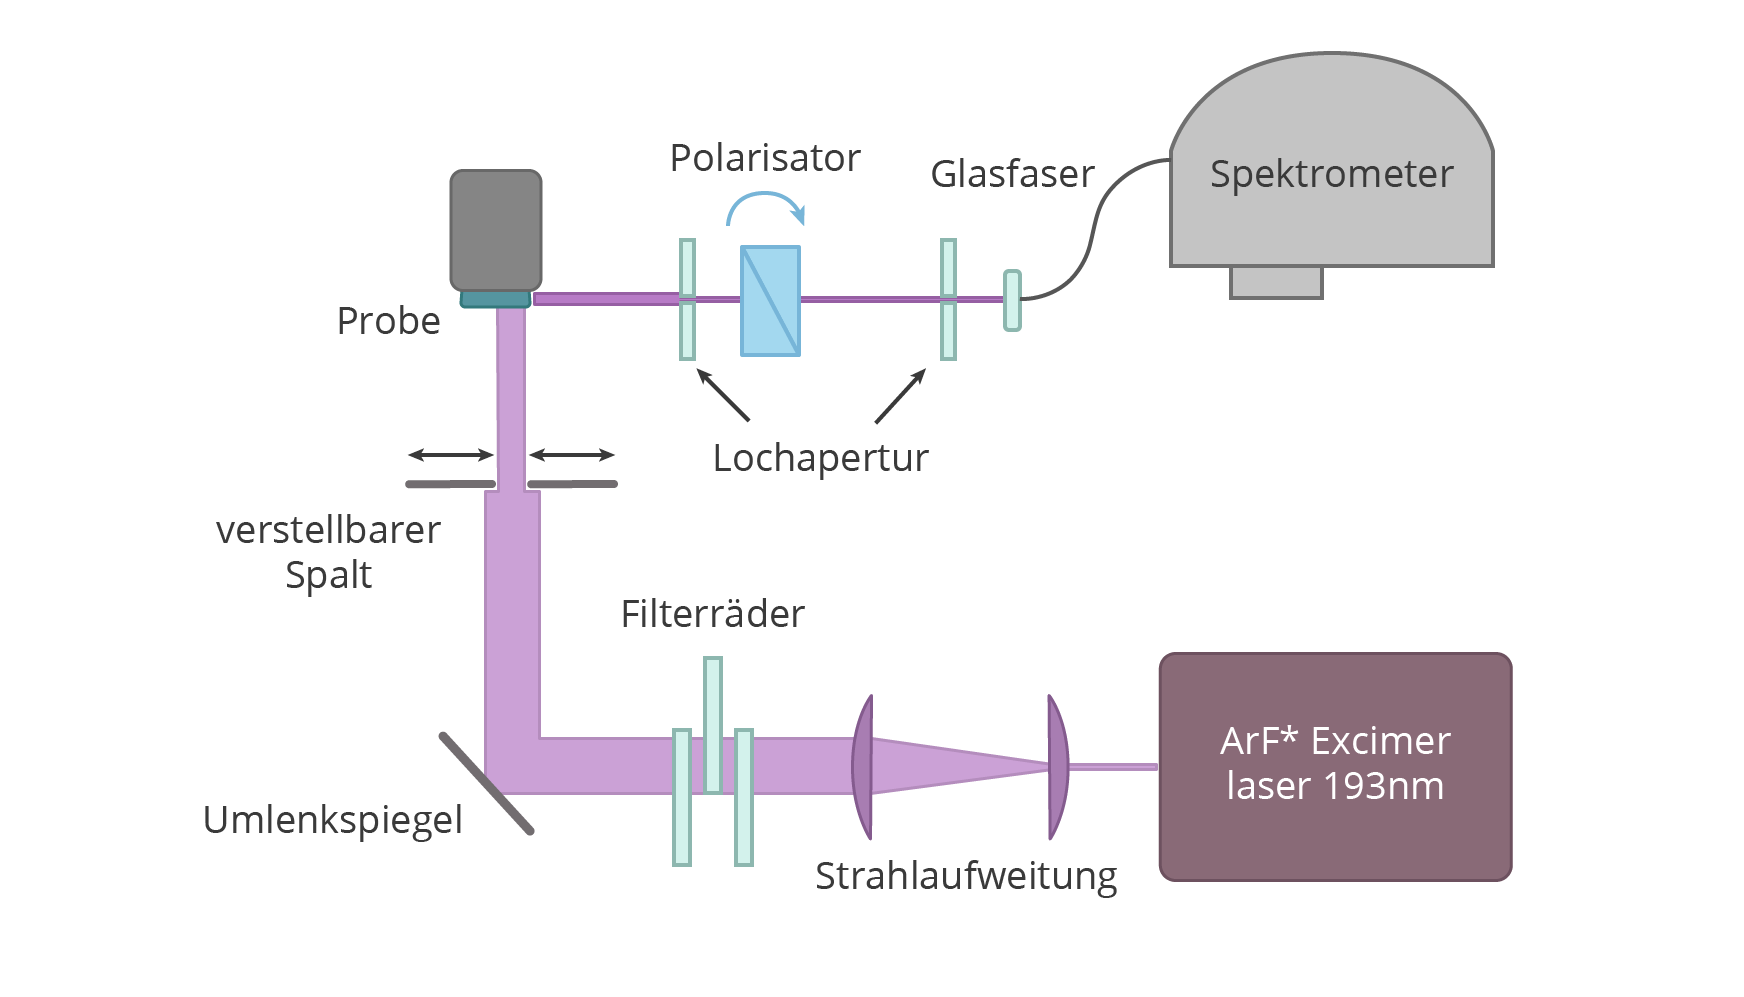
\includegraphics[width=0.8\linewidth]{Bilder/aufbauPol.png}
        \caption{Aufbau des Photolumineszenzmessplatzes der AG Kneissl zur Bestimmung der Polarisation. }
        \label{fig:polaufbau}
    \end{minipage}% <- sonst wird hier ein Leerzeichen eingefügt
\end{figure}
\vspace{1cm}
\noindent
Der Messaufbau zur Bestimmung der Lichtpolarisation ist in Abbildung \ref{fig:polaufbau} dargestellt.
Die Anregung der untersuchten Proben erfolgt senkrecht zur Probenoberfläche. Die Lumineszenz der Probe wird aus der Kante gemessen, weil TM-polarisiertes Licht nur vertikal zur c-Achse, wie in Abbildung \ref{fig:martintetm} sichtbar, emittiert wird. Die Lumineszenz wird dann unter kleinem Öffnungswinkel über eine Linse mit sich dahinter befindlicher Blende eingesammelt und parallelisiert. Das parallelisierte Licht wird dann durch einen Glan-Taylor-Polarisator geleitet. Dass das Licht parallelisiert ist, ist wegen der anisotropen Brechzahl des Polarisators wichtig. Diese ist neben der Polarisationsrichtung auch von dem Eintrittswinkel abhängig und entscheidet ob der Strahl transmittiert oder reflektiert wird \cite{0950-7671-25-12-304}. In Abhängigkeit der Orientierung des Polarisators wird TE- oder TM-polarisiertes Licht transmittiert. Der eingestellte Winkel lässt sich $1^\circ$ granular einstellen. 

	\chapter{Aufbau: Erweiterung und Bestimmung der Degradation des UV Quarzglases }
\thispagestyle{fancy}

\section{Bestimmung der Degradation des UV Quarzglases}
%
\begin{figure}[htb]
  \centering
  \begin{minipage}[t]{0.49\linewidth}
      \centering
      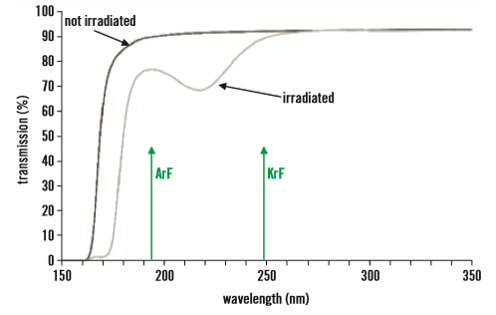
\includegraphics[width=\linewidth]{Bilder/uvsilicaDegradation.png}
      \caption{Vom Hersteller angegebene wellenlängenabhängige Transmission vor und nach Degradation durch Bestrahlung.}
      \label{fig:degra}
  \end{minipage}
\end{figure}
\vspace{1cm}
\raggedright
Da die Messung der Anregungsleistungdichte erfolgt, bevor das Laserlicht die Probe durch das UV-Quarzglas im Kryostaten trifft, ist es wichtig den Transmissionsverlust zu bestimmen, um die realen Werte für die Anregungsleistungsdichte zu kennen (Die Anregungsleistungsdichte die bei der Probe ankommt). Der Kryostat besitzt vier Fenster, bestehend aus UV-Quarzglas, das besonders transparent im UV-Wellenlängen bereich ist. Durch diese Fenster dringt das Laserlicht in den Probenhalter ein. Von diesen Fenstern war und ist eines in dauerhaftem Gebrauch. Wie in Abb. ~\ref{fig:degra} zu sehen ist, weisen die Fenster aber mit der fortlaufender Bestrahlung Degradation auf, so nimmt laut Hersteller durch Degradation die Transmission von 90 Prozent bis auf ca. 75 Prozent ab für eine Wellenlänge von 193 nm.
Um nun den Transmissongrad zu bestimmen, wurde der Probenhalter aus dem Kryostat entfernt, damit das Laserlicht ungehindert durch zwei parallel liegende Fenster durchdringen kann, um so auch die Anregungsleistungsdichte des Laserlichtes nach durchdringen des letzten Fenster messen zu können. So konnte die Anregungsleistungsdichte vor dem Eintreten und nach dem Austreten in den Kryostaten bestimmt werden. 
Dies wurde einmal bei den parallel liegenden unbenutzten Fenstern gemacht. Davon ausgehend, dass beide Fenster, da unbenutzt, den gleichen Transmissionsgrad haben, kann darauf zurückgeschlossen werden, dass ein unbenutztes Fenster einen Transmissionsgrad von 59 Prozent aufweist, was um ca. 10 Prozent von der Herstellerangabe abweicht, die aber nicht die Reflektion im Kryostaten mitberechnet. 
%
\begin{figure}[htb]
  \centering
  \begin{subfigure}{0.40\textwidth}
    \centering
    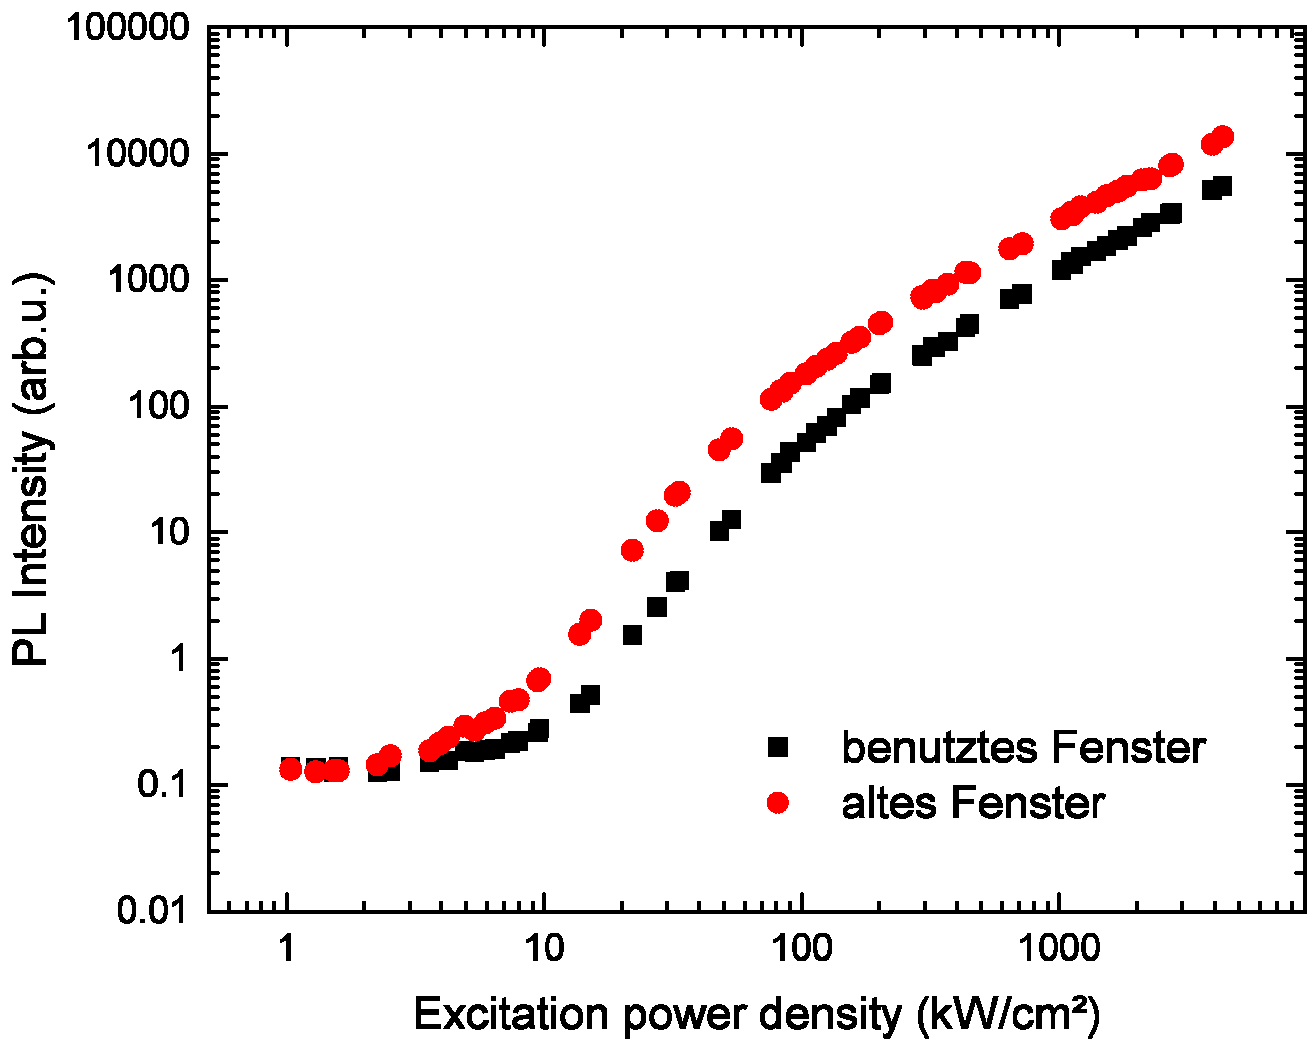
\includegraphics[width=0.9\linewidth]{Bilder/uvsilicavergleich.pdf}
    \caption{PL Intensität in Abhängigkeit der Anregungsleistungsdichte mit den benutzten und unbenutzten Fenstern}
    \label{fig:sub1}
  \end{subfigure}%
  {\LARGE$\xrightarrow{\cdot 0,44}$}
  \begin{subfigure}{0.40\textwidth}
    \centering
    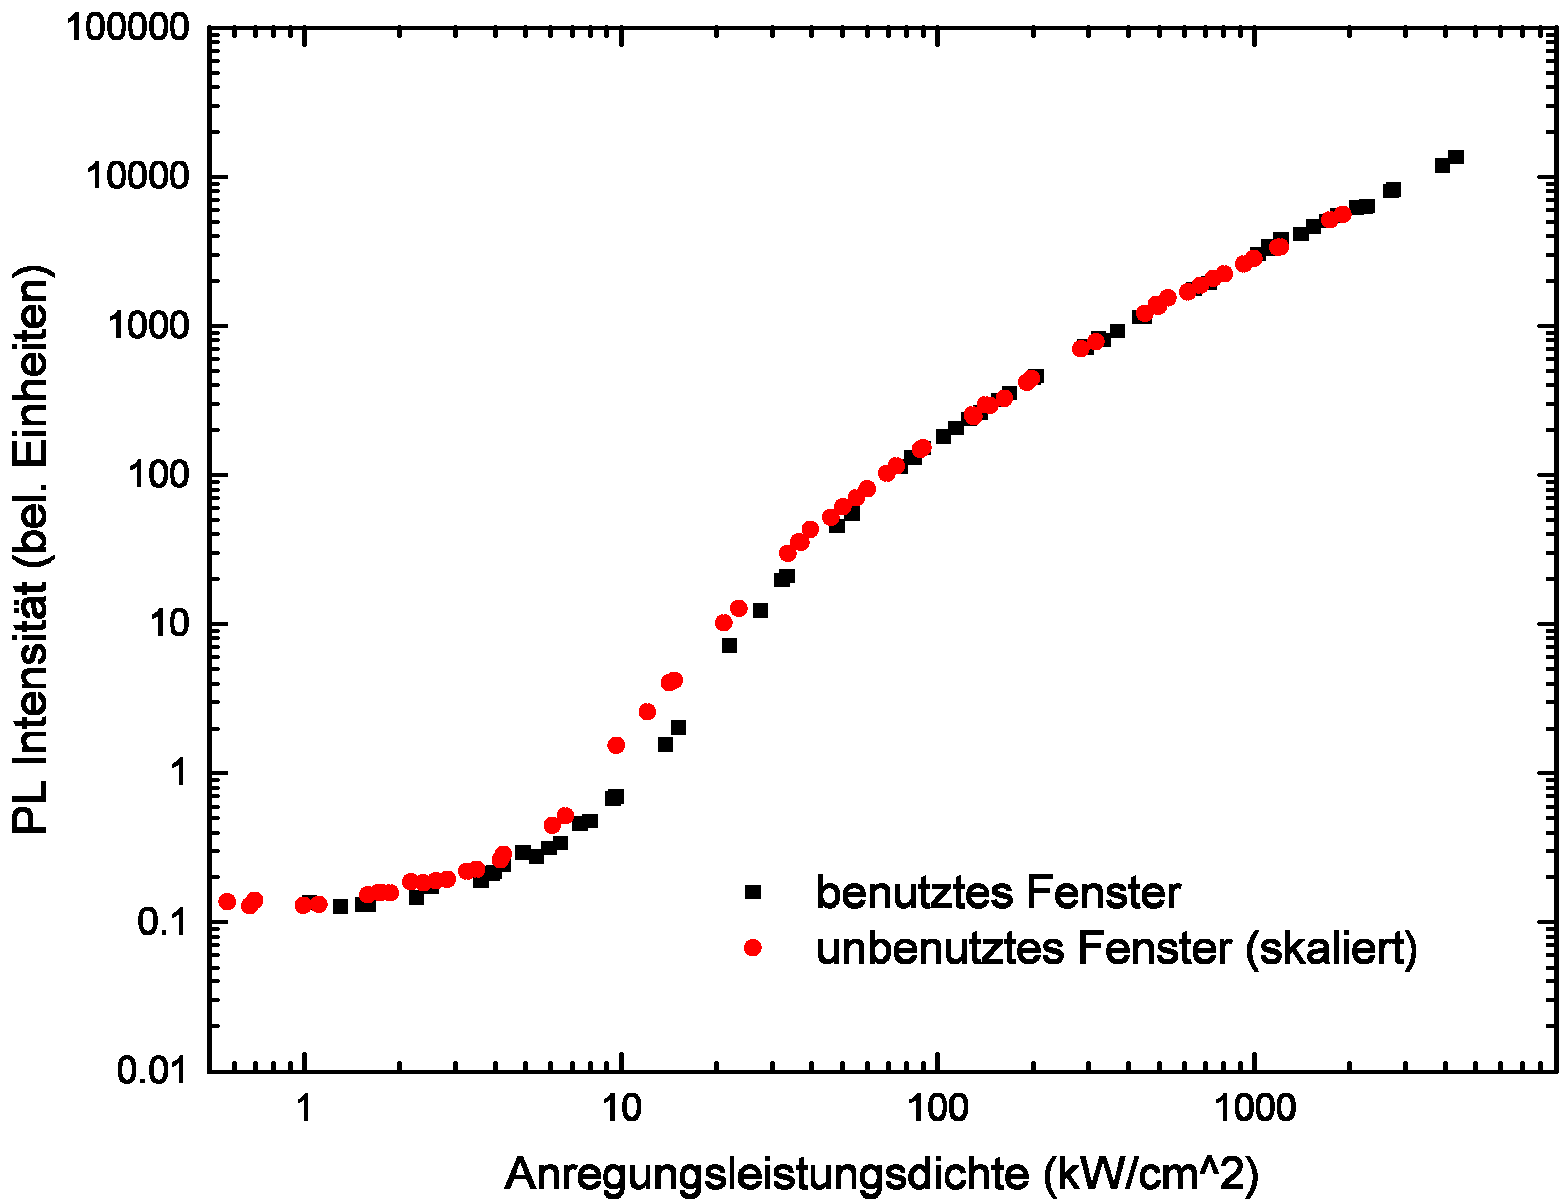
\includegraphics[width=0.9\linewidth]{Bilder/uvsilicaVergleichSkaliert.pdf}
    \caption{Die Anregungsleistungsdichte des unbenutzten Fensters mit den rechnerisch bestimmten 0,44 skaliert}
    \label{fig:sub2}
  \end{subfigure}
  \caption{}
  \label{fig:vergleichSkaliert}
\end{figure}
%
Um den Transmissionsgrad des benutzten Fensters zu bestimmen, wurde die Transmission durch das benutzte Fenster und dem parallel liegenden unbenutzten Fenster gemessen. Mit dem Wissen, dass der Transmissionsgrad durch das unbenutzte Fensters bei 59 Prozent ($T_{unb} = 0,59$), kann die Transmission durch das benutzte Fenster auf 26 Prozent ($T_{ben} = 0,26$) runtergerechnet werden. 
Davon ausgehend, dass die Transmission bei höheren Wellenlängen (Emission) gleich und bei beiden Fenstern ähnlich ist,
%
\begin{equation}
  F_{skal} = \frac{ T_{ben} }{ T_{unb} } = 0,44\label{eq11}
\end{equation}
%
kann der Skalierungsfaktor mit für die Anregungsleistungsdichte auf 0,44 bestimmt werden. Was bedeutet, dass durch Degradation die Transmission auf 44 Prozent der ursprünglichen Transmission gesunken ist.
Dies bestätigt sich auch durch die Gegenüberstellung in Abb. ~\ref{fig:vergleichSkaliert}. Dies bedeutet, dass durch die zeitliche Degradation die Transmission auf 44 Prozent der ursprünglichen gesunken ist.
Im Umkehrschkuss bedeutet dies, dass von der Anregungsleistungsdichte durch die geringe Transmission der Fenster und Reflektion im und außerhalb des Kryostaten nur ca. 26 Prozent bei der Probe ankommen. 
	\section{Aufbau: Erweiterung der Filterkombinationen}
\thispagestyle{fancy}

Im Zuge dieser Arbeit wurden für eine Erhöhung der Messpunkte und Verringerung von Rauschen bei der leistungsdichteabhängigen Messung der IQE die Anzahl der Filterkombination erhöht. Dafür wurden die alten zwei Filterräder durch drei neue ersetzt. 
%
\begin{figure}[ht!]
    \centering
    \begin{minipage}[t]{1\linewidth}
        \centering
        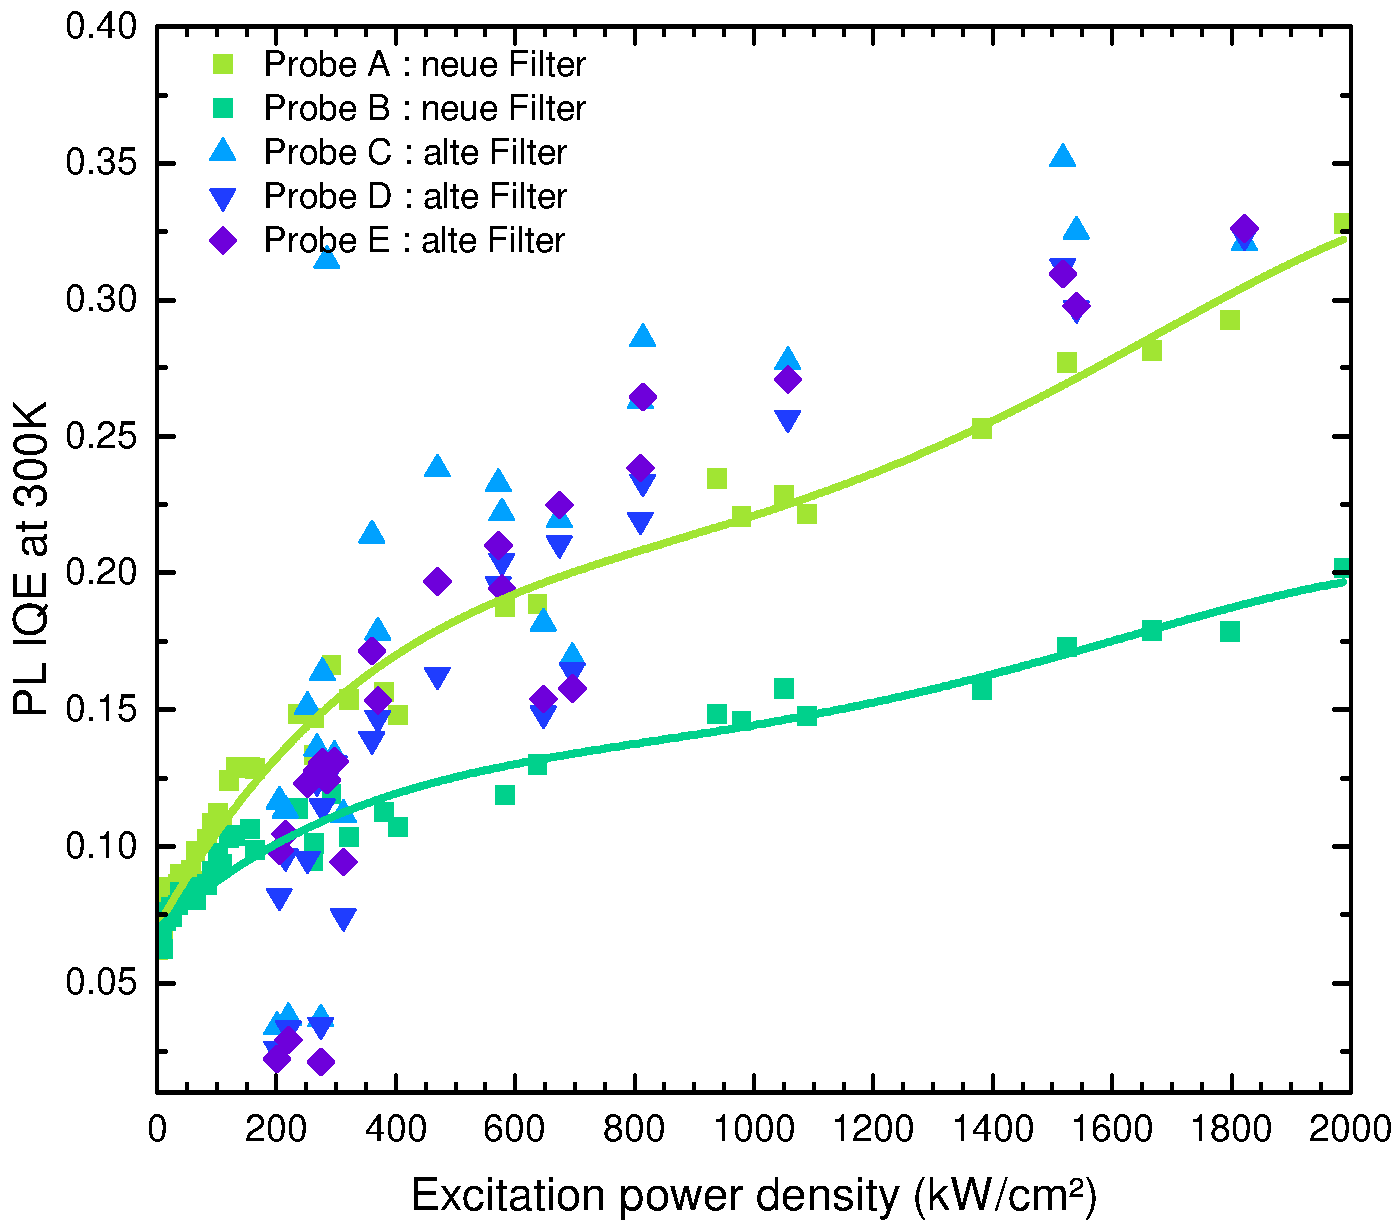
\includegraphics[width = 0.49\linewidth]{Bilder/AuswertungNovemeberKorr1VergleichFilter.pdf}
        \caption{Vergleich der Messung von insgesamt 5 ähnlichen Proben. 3 Proben (blau) wurden mit dem alten Setup gemessen. 2 Proben (grün, durchgezogene Linie) wurden mit dem neuen Setup gemessen. Die Präzision in tieferen Anregungsleistungsdichtenbereichen ist für das neue Setup deutlich erhöht. Das Rauschen fällt ebenfalls deutlich geringer aus. }
        \label{fig:vergleichFilter}
    \end{minipage}
\end{figure}
%
\newpage
Durch die erhöhte Anzahl möglicher Filterkombinationen ist es möglich, statt nur 27 verschiedene Messpunkte 61 zu nehmen. Speziell der Bereich der geringen Anregungsleistungsdichten kann so besser aufgelöst werden und das Rauschen wurde im Allgemeinen stark verringert \ref{fig:vergleichFilter}. 
%


	\chapter{Ergebnisse}
\thispagestyle{fancy}
\section{Untersuchung optisch gepumpter Laserstrukturen auf unterschiedlichen Templates}


Dieses Kapitel widmet sich der Untersuchung der beiden Probenreihen TS4045 und TS4048 von optisch gepumpten Laserstrukturen die aus Rezepten aus zwei unterschiedlichen Serien stammen. Die beiden Serien unterscheiden sich im wesentlichen dadurch, dass sie mit(TS4048) und ohne Übergitter(TS4045) gewachsen wurden. Jede Reihe für sich weist  zusätzlich noch Unterschiede den Proben selbst auf, so sind zwei Proben der Reihe TS4045 auf AlN-Bulk zweier unterschiedlicher Hersteller (HexaTech, IKZ) gewachsen und alle  anderen Proben auf ELO AlN/Sapphire mit jeweils 3 unterschiedlichen "offcut"-Winkeln. Tabellerisch sieht die  Zusammenstellung wie folgt aus: 

\vspace{1cm}


\setlength{\arrayrulewidth}{0.5mm}
\setlength{\tabcolsep}{0.5pt}
\renewcommand{\arraystretch}{1.5}
 

\begin{tabular}{ |c|c|c|c|c|c|   }
\hline
\multicolumn{3}{|c|}{TS4045} & \multicolumn{3}{c|}{TS4048}  \\
\hline
Endung & offcut& Template & Endung & offcut& Template \\
\hline
-2V* & 0.1$^\circ$m & ELO & -2V* & 0.1$^\circ$m & ELO \\
-2H & 0.1$^\circ$m & ELO & -2H & 0.1$^\circ$m & ELO \\
-2Z & 0.2$^\circ$m & ELO & -1 & 0.1$^\circ$m & ELO \\
-1 & 0.1$^\circ$m & Bulk(IKZ) & -2V* & 0.1$^\circ$m & ELO \\
-3* & 0.1$^\circ$m & Bulk(Hexatech) & -2V* & 0.1$^\circ$m & ELO \\
\hline



\end{tabular}




	\bibliography{Bibliographie}
\end{document}	


\begin{comment}
	\begin{figure}[b!]
    		
\includegraphics[width=0.2\textwidth]{Bilder/TU-Berlin-Logo.pdf}
    		\label{fig:tulogo}
    	\end{figure}	
\end{comment}	
